\documentclass[12pt]{article}

%Packages BEGIN
\usepackage{amsmath}
\usepackage{physics}
\usepackage{float}
\usepackage{graphicx}
\usepackage{booktabs}

%Packages END

\title{CA Final Project - Report}
\author{B07202020 Hao-Chien Wang\\B07901135 Guo-Wei Ho}

\begin{document}
\maketitle

\section{Design}%
\label{sec:design}

\begin{figure}[h!]
	\centering
	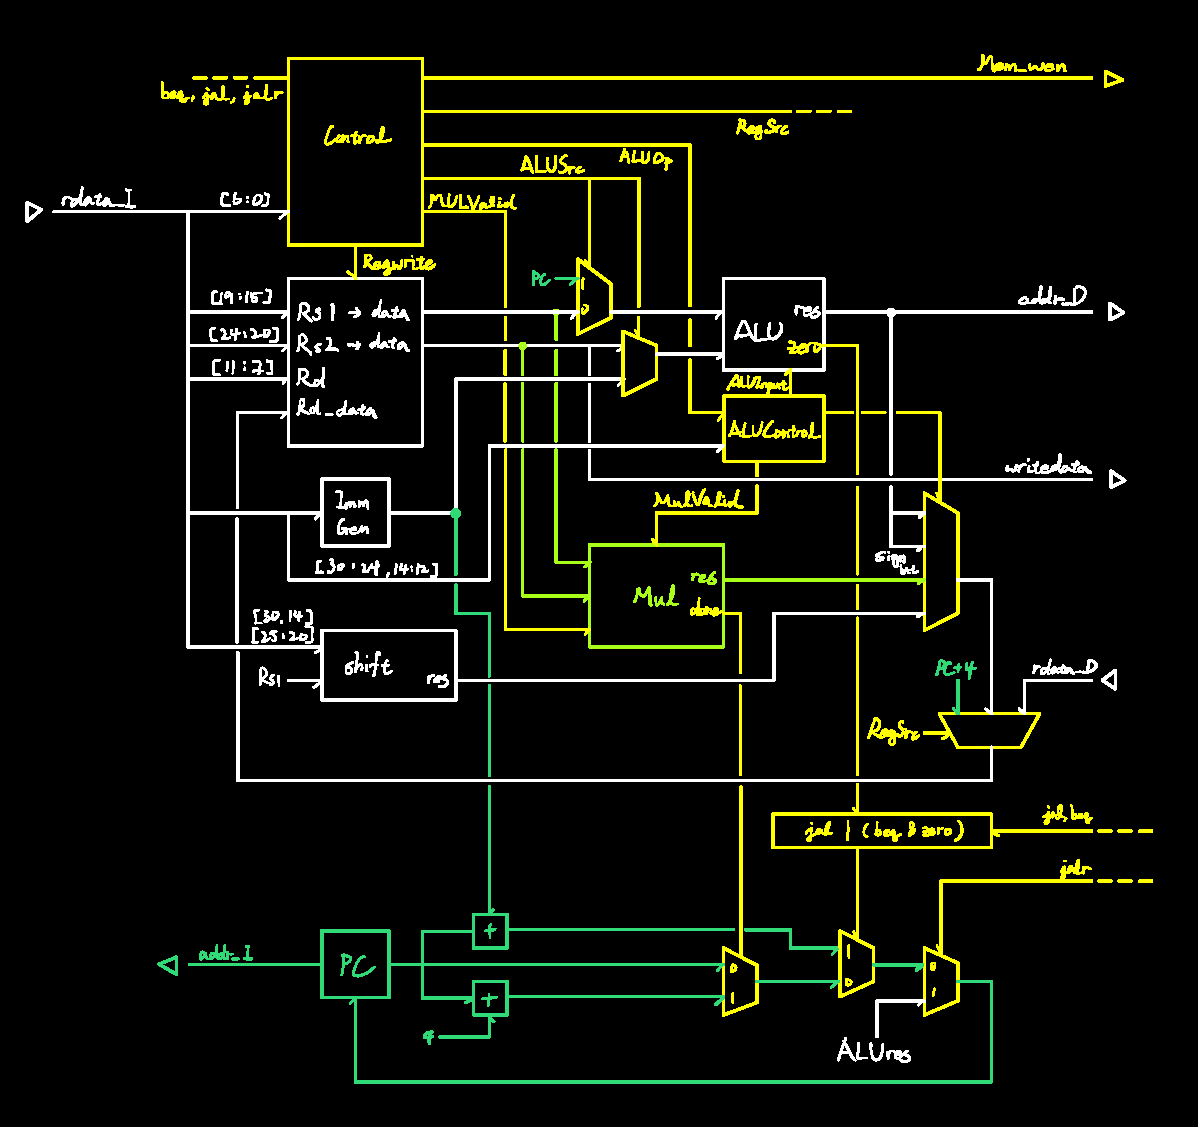
\includegraphics[width=\linewidth]{./CA-Final-Project-Design-crop.pdf}
	\caption{CPU design}%
	\label{fig:design}
\end{figure}


Our design is drawn in figure \ref{fig:design}, which is mostly identical to the
design in the textbook, but a few modules, signals and wires are added to support
more instructions. \\

\subsection{The Control Module}%
\label{sub:the_control_module}


\indent The control module reads the \texttt{opcode}, and output 9 signals:
\begin{itemize}
	\item \texttt{Regwrite}: 1-bit signal.\texttt{1} if writing to register is 
		required, \texttt{0} otherwise.

	\item \texttt{ALUSrc}: 2-bit signal, one for each ALU input. The input will
		be from the register if the signal is \texttt{0}. The first input will
		be from PC, and the other input will be from the \texttt{ImmGen} if the
		corresponding signals are \texttt{1}.

	\item \texttt{ALUOp}: 2-bit signal. Indicates the instruction type to help
		ALU control further decides the operation of ALU. The signals are defined
		as follows:
		\begin{itemize}
			\item \texttt{00}: always add.
			\item \texttt{01}: always subtract.
			\item \texttt{10}: R-type intruction. Operation depends on funct7.
			\item \texttt{11}: R-type intruction. Operation depends on funct7.
		\end{itemize}

	\item \texttt{RegSrc}: 2-bit signal. Together with \texttt{ALURegSrc}, they
		determine the source written back to the register. The meanings of each
		signals are:
		\begin{itemize}
			\item \texttt{00}: ALU
			\item \texttt{01}: $\text{PC}+4$
			\item \texttt{10}: Memory
		\end{itemize}

	\item \texttt{Mem\_wen}: 1-bit signal, \texttt{1} for writing the memory,
		\texttt{0} otherwise.

	\item \texttt{beq}: 1-bit signal, signaling the branch instruction.
	\item \texttt{jal}: 1-bit signal, signaling the \texttt{jal} instruction.
	\item \texttt{jalr}: 1-bit signal, signaling the \texttt{jalr} instruction.

\end{itemize}

The signals for each instructions are listed in table \ref{tab:control}.

\begin{table}[h]
\centering
\begin{tabular}{@{}lllllll@{}}
\toprule
Intruction     & \texttt{opcode}           & \texttt{men\_wen\_D}  & \texttt{RegSrc}       & \texttt{ALUop}       & \texttt{ALUSrc}      & \texttt{Regwrite}   \\ \midrule
\texttt{lw}    & \texttt{0000011} & \texttt{0} & \texttt{10} & \texttt{00} & \texttt{01} & \texttt{1} \\
\texttt{addi}  & \texttt{0010011} & \texttt{0} & \texttt{00}   & \texttt{11} & \texttt{01} & \texttt{1} \\
\texttt{slli}  & \texttt{0010011} & \texttt{0} & \texttt{00}   & \texttt{11} & \texttt{01} & \texttt{1} \\
\texttt{slti}  & \texttt{0010011} & \texttt{0} & \texttt{00}   & \texttt{11} & \texttt{01} & \texttt{1} \\
\texttt{srai}  & \texttt{0010011} & \texttt{0} & \texttt{00}   & \texttt{11} & \texttt{01} & \texttt{1} \\
\texttt{auipc} & \texttt{0010111} & \texttt{0} & \texttt{00} & \texttt{00} & \texttt{11} & \texttt{1} \\
\texttt{sw}    & \texttt{0100011} & \texttt{1} & \texttt{X}   & \texttt{00} & \texttt{01} & \texttt{0} \\
\texttt{add}   & \texttt{0110011} & \texttt{0} & \texttt{00}   & \texttt{10} & \texttt{00} & \texttt{1} \\
\texttt{sub}   & \texttt{0110011} & \texttt{0} & \texttt{00}   & \texttt{10} & \texttt{00} & \texttt{1} \\
\texttt{mul}   & \texttt{0110011} & \texttt{0} & \texttt{00}   & \texttt{10} & \texttt{00} & \texttt{1} \\
\texttt{beq}   & \texttt{1100011} & \texttt{0} & \texttt{X}   & \texttt{01} & \texttt{00} & \texttt{0} \\
\texttt{jalr}  & \texttt{1100111} & \texttt{0} & \texttt{01}   & \texttt{00} & \texttt{01} & \texttt{1} \\
\texttt{jal}   & \texttt{1101111} & \texttt{0} & \texttt{01}   & \texttt{X}  & \texttt{X}  & \texttt{1} \\
DEFAULT        &                  & \texttt{0} & \texttt{000} & \texttt{00} & \texttt{00} & \texttt{0} \\ \bottomrule
\end{tabular}
\caption{Control signals of each instructions.}
\label{tab:control}
\end{table} 

\subsection{The ALU Control}%
\label{sub:the_alu_control}

The ALU control decides the operation of the ALU, and also plays a part in
determining the source written back to the register. This module takes 
\texttt{ALUOP}, \texttt{funct3} and \texttt{funct7} and several output sources
as inputs (explained below in the \texttt{ALURegSrc} part), then output
\texttt{ALUInput} to the ALU to control the operation of the ALU,  
\texttt{ALURegSrc} to the multiplexer determining the source written back, and
\texttt{MulValid} to trigger the multiplication.

\begin{itemize}
	\item \texttt{ALUInput}: 3-bit signal. Determines the operation of the ALU.
		\begin{itemize}
			\item \texttt{010}: add
			\item \texttt{110}: subtract
		\end{itemize}
		Note that we use 3 bits instead of one, even though there are really
		two options. The advantage is that it can easily be modified to support 
		more operatios such as \texttt{and}, \texttt{or}, etc.


    \item \texttt{ALUMUX}: Takes the results of ALU, Multiplier, and Shift Unit, and assign
        the desired result to \texttt{ALURegSrc}. Note that we implement this unit
        along with \texttt{ALUInput} and consider it a part of \texttt{ALUControl} 
        since the output also depends on \texttt{ALUOp}, \texttt{funct3}, and \texttt{funct7}. 
        
    \item \texttt{ALURegSrc}: 32-bit data bus. The result from ALU, Multiplier, or Shift Unit to
        \texttt{rd\_data} (including the sign bit for the instruction \texttt{STLI})

	\item \texttt{MulValid}: 1-bit signal. \texttt{1} if the intruction is
		\texttt{mul}, 0 otherwise. The details about multiplication will be described
		in section \ref{sub:multiplication}.
\end{itemize}

\subsection{Multiplication}%
\label{sub:multiplication}

The mulitiplication module is from HW3. The output signal \texttt{done} is 
\texttt{1} unless \texttt{MulValid} is \texttt{1} and the multiplication state
is not in \texttt{S\_DONE}. \texttt{done} controls the PC. When \texttt{done} is
\texttt{0}, the PC is frozen (the next state of PC is the same as the present state).
Otherwise it is $\text{PC}+4$ as usual. This means when instruction is \texttt{mul},
the ALU control unit set \texttt{mulValid} to 1, and the multiplication process
is triggered. During the process the \texttt{done} signal is \texttt{0} until
the result is ready. Before that the PC is frozen, which means all the modules
are also frozen except the multiplication module. When the result is ready, the
state is in \texttt{S\_DONE} and \texttt{done} is set back to 1, and PC goes 
on to the next instruction.

\section{Extra Instructions Datapath}

    

\section{Required Screenshots}%
\label{sec:required_screenshots}

\begin{figure}[H]
	\centering
	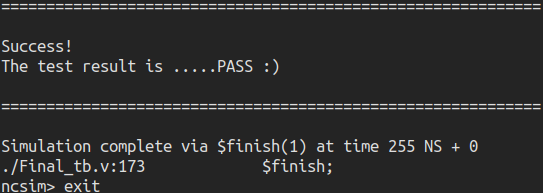
\includegraphics[width=\linewidth]{./leaf.png}
	\caption{Simulation time of \textit{leaf example}.}%
	\label{fig:leaf}
\end{figure}

\begin{figure}[H]
	\centering
	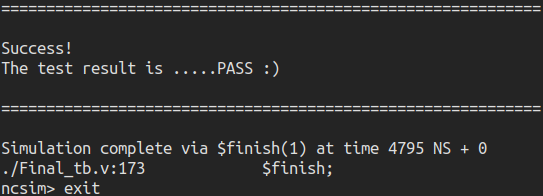
\includegraphics[width=\linewidth]{./fact.png}
	\caption{Simulation time of \textit{fact}.}%
	\label{fig:fact}
\end{figure}

\begin{figure}[H]
	\centering
	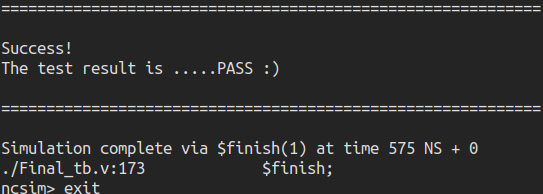
\includegraphics[width=\linewidth]{./hw1.png}
	\caption{Simulation time of \textit{HW1}.}%
	\label{fig:hw1}
\end{figure}

\begin{figure}[H]
	\centering
	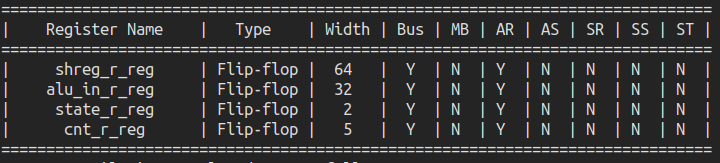
\includegraphics[width=\linewidth]{./ff.png}
	\caption{Coding style check.}%
	\label{fig:ff}
\end{figure}

\section{Work Distribution}%
\label{sec:work_distribution}

\begin{itemize}
	\item Hao-Chien Wang: Control, ALU, ALUControl, debug, report.
	\item Guo-Wei Ho: Design, instruction generation, ImmGen, multiplier (HW3), multiplexers, all other little stuff, debug.
\end{itemize}


\end{document}
